%% Figure snippets produced by plot-agent for inclusion in main.tex.
%% All numerical values in data-grounded figures trace to experimental_log.md.

% Figure 1 (data-grounded): Firing rates across conditions
\begin{figure}[htbp]
\centering
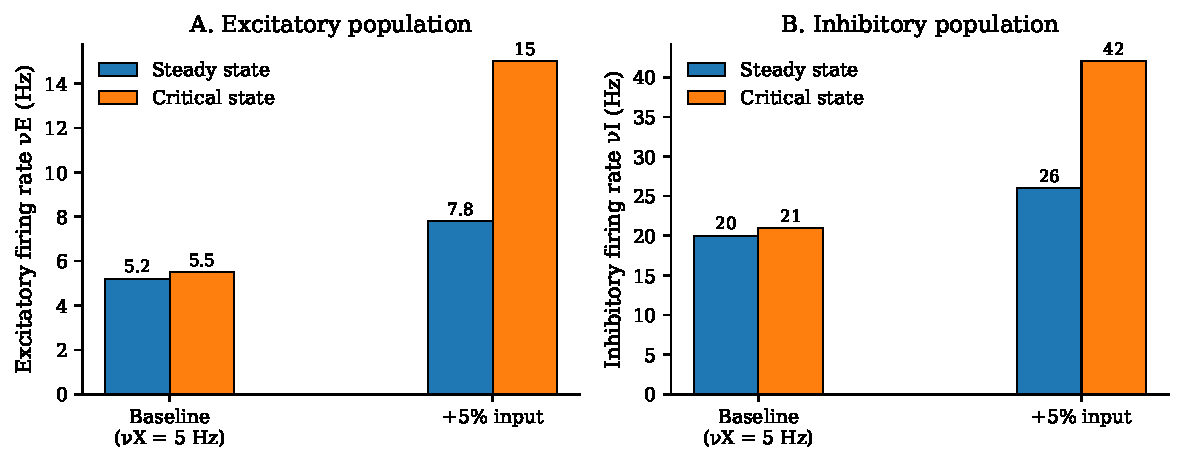
\includegraphics[width=0.95\textwidth]{figures/fig_firing_rates.pdf}
\caption{Firing rates of excitatory ($\nu_E$) and inhibitory ($\nu_I$)
populations in the steady state and critical state primary networks.
\textbf{A.}~Excitatory rates: 5.2 Hz (steady, baseline), 5.5 Hz (critical,
baseline), 7.8 Hz (steady, $+5\%$ input), 15 Hz (critical, $+5\%$ input).
\textbf{B.}~Inhibitory rates: 20 Hz (steady, baseline), 21 Hz (critical,
baseline), 26 Hz (steady, $+5\%$ input), 42 Hz (critical, $+5\%$ input).
The steady state network shows graded rate increases while the critical
state network undergoes a qualitative transition to the oscillatory regime.}
\label{fig:firing_rates}
\end{figure}

% Figure 2 (data-grounded): Model vs experiment comparison
\begin{figure}[htbp]
\centering
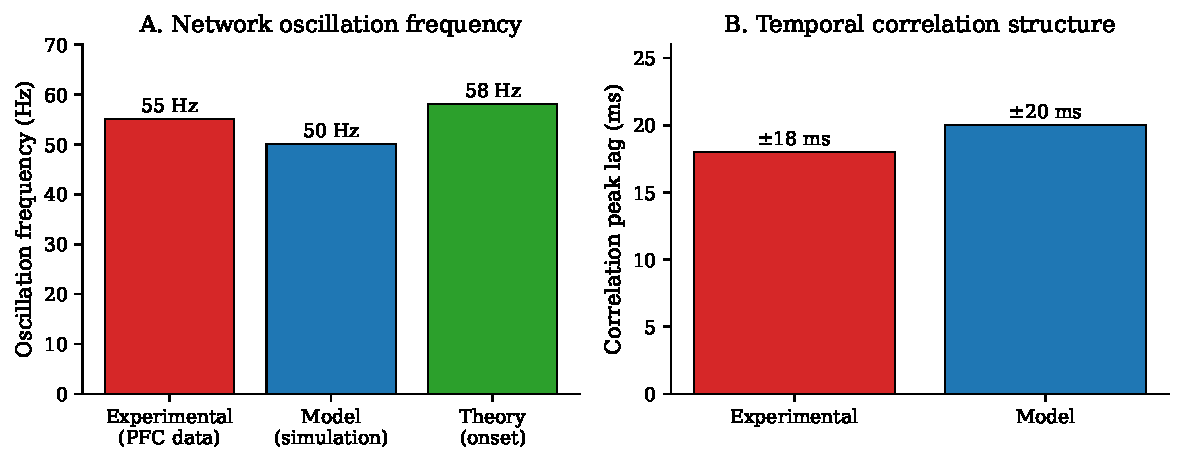
\includegraphics[width=0.95\textwidth]{figures/fig_model_vs_experiment.pdf}
\caption{Quantitative comparison between simulation and experimental data.
\textbf{A.}~Network oscillation frequencies: experimental value $\sim$55 Hz
from monkey PFC \citep{zick2018blocking}, simulated value $\sim$50 Hz, and
theoretically predicted onset frequency 58 Hz. \textbf{B.}~Temporal
correlation peak lags: $\pm$18 ms (experimental) and $\pm$20 ms (model),
both consistent with gamma-frequency periodicity.}
\label{fig:model_vs_experiment}
\end{figure}

% Figure 3 (schematic): Network architecture
\begin{figure}[htbp]
\centering
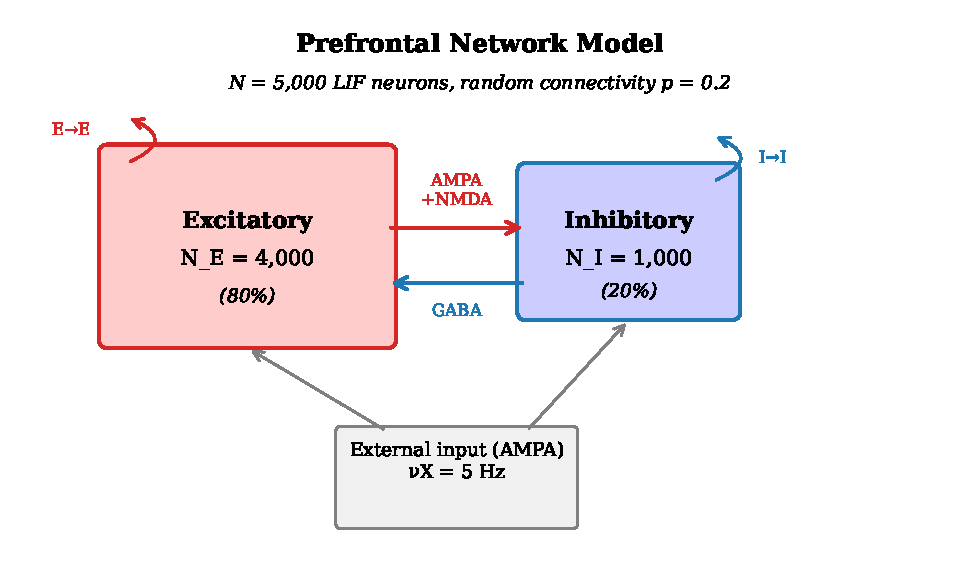
\includegraphics[width=0.75\textwidth]{figures/fig_network_schematic.pdf}
\caption{Architecture of the prefrontal network model. $N = 5{,}000$ leaky
integrate-and-fire neurons partitioned into $N_E = 4{,}000$ (80\%) excitatory
and $N_I = 1{,}000$ (20\%) inhibitory populations connected randomly with
probability $p = 0.2$. Excitatory recurrent connections are mediated by
both AMPA and NMDA receptors, inhibitory connections by GABA receptors, and
all neurons receive external AMPA input at baseline rate $\nu_X = 5$ Hz.}
\label{fig:schematic}
\end{figure}

% Figure 4 (schematic): State diagram
\begin{figure}[htbp]
\centering
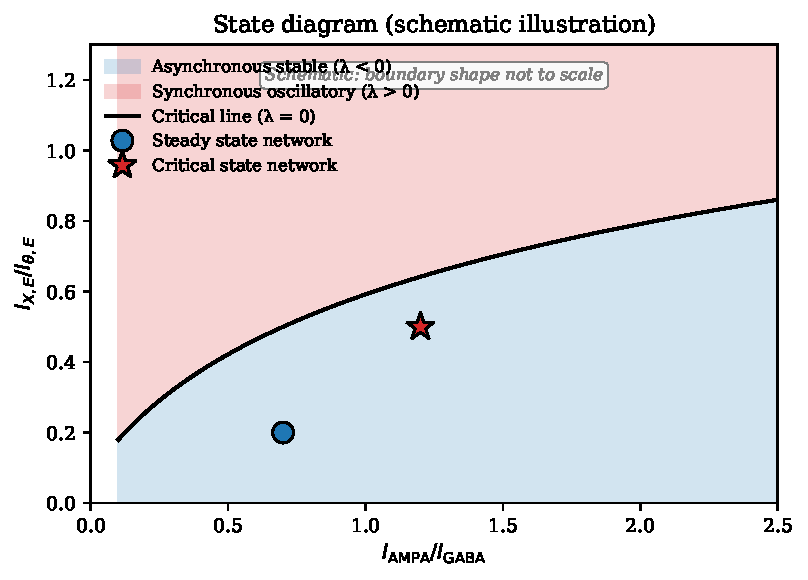
\includegraphics[width=0.65\textwidth]{figures/fig_state_diagram.pdf}
\caption{Schematic state diagram in the
$(I_{\mathrm{AMPA}}/I_{\mathrm{GABA}}, I_{X,E}/I_{\theta,E})$ parameter
plane, based on linear stability analysis with external input rate
$\nu_X = 5$ Hz and NMDA-to-GABA current balance
$I_{\mathrm{NMDA}}/I_{\mathrm{GABA}} = 0.2$. The asynchronous stationary
state ($\lambda < 0$) is stable below the critical line, and synchronous
oscillation ($\lambda > 0$) emerges above it. The steady state primary
network (blue circle) and critical state primary network (red star)
differ in their proximity to the oscillatory boundary. Boundary shape is
illustrative.}
\label{fig:state_diagram}
\end{figure}
